%
\documentclass[tikz]{standalone}

\usepackage{tikz}
\usetikzlibrary{calc}
\usetikzlibrary{lindenmayersystems}



\usetikzlibrary{trees,snakes}
\tikzstyle{level 1}=[sibling angle=30, level distance=1cm]
\tikzstyle{level 2}=[sibling angle=20, level distance=.7cm]
\tikzstyle{level 3}=[sibling angle=10, level distance=.49cm]
\tikzstyle{every node}=[%fill,
		 				inner sep=0pt]
%\tikzstyle{edge from parent}=[snake=ticks,segment length=2mm,draw]
\tikzstyle{edge from parent}=[draw]



\begin{document}
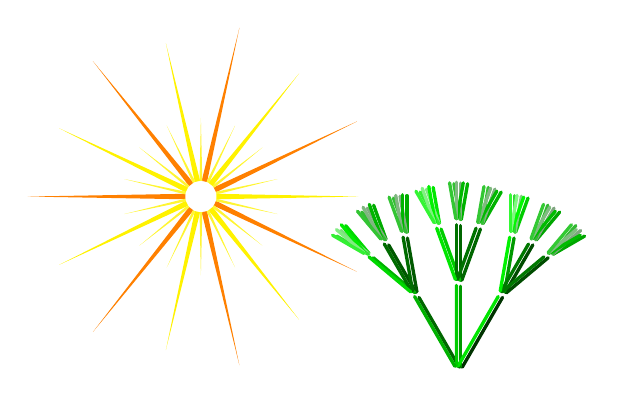
\begin{tikzpicture}



%% Zweig
\begin{scope}[xshift=3.3cm,yshift=-2.2cm, scale=1.1]

\begin{scope}[grow cyclic,shape=circle,very thick, cap=round, rotate=90] 
\node at (0,0) {} child [color=\A] foreach \A in {green!20!black,green!60!black,green!40!black}
    { node {} child [color=\A!50!\B] foreach \B in {green!50!black,green!50!black,green}
        { node {} child [color=\A!50!\B!50!\C] foreach \C in {green,white,green!80}
            { node {} }
        }
    };
\node at (0.01,0.05) {} child [color=\A] foreach \A in {green!90!black,green!80!black,green!70!black}
    { node {} child [color=\A!50!\B] foreach \B in {green!50!black,green!50!black,green}
        { node {} child [color=\A!50!\B!50!\C] foreach \C in {green,white,green!80}
            { node {} }
        }
    };
\end{scope}
\end{scope}


%% Star

\newcommand{\drawstar}[1]{
\foreach \i in {1,...,\nstar}{
	\pgfmathsetmacro{\ang}{360*\i/\nstar+\rot}
	\path (C)++(\ang+\dangi:\Ri) coordinate(L);
	\path (C)++(\ang-\dangi:\Ri) coordinate(R);
	\path[fill=#1] (L)--($(C)+(\ang:\Ro)$) -- (R);
}}



\path (0,0) coordinate(C);
\def\nstar{7}
\def\Ri{.2}
\def\Ro{2}
\def\dangi{10}
\def\rot{0}
\drawstar{yellow};

\def\Ro{2.2}
\pgfmathsetmacro{\rot}{360/7/2}
\drawstar{orange};

\def\nstar{14}
\def\Ro{1}
\def\dangi{5}
\pgfmathsetmacro{\rot}{360/7/4}
\drawstar{yellow!80};









\end{tikzpicture}
\end{document} 
